% Source of the figure counterexample-cut-two.pdf: a graph with c(u,v) = 2 and d(u,v) = 3 in which the red
% u-v path is a u-v cut. Compile with pdfLaTeX; the PDF is included in the manuscript at its natural size.
\documentclass[tikz,border=1pt]{standalone}
\usepackage[T1]{fontenc}
\usepackage{stix}
\pdfinfoomitdate=1 \pdftrailerid{} \pdfsuppressptexinfo=-1
\definecolor{pathred}{RGB}{200,40,40}
\begin{document}
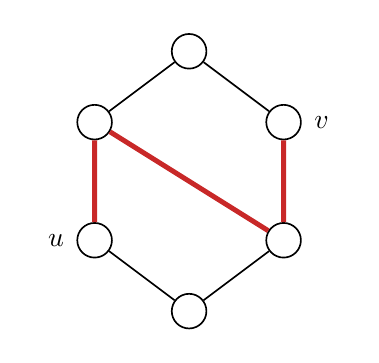
\begin{tikzpicture}[x=1cm, y=1cm,
    vertex/.style={circle, draw, fill=white, line width=0.6pt, inner sep=0pt, minimum size=4.4mm},
    edge/.style={line width=0.6pt},
    pathedge/.style={line width=1.8pt, pathred}]
  \useasboundingbox (-0.85,-1.2) rectangle (3.25,2.7);
  \node[vertex] (t) at (1.2,2.4) {};
  \node[vertex] (a) at (0,1.5) {};
  \node[vertex] (v) at (2.4,1.5) {};
  \node[vertex] (u) at (0,0) {};
  \node[vertex] (b) at (2.4,0) {};
  \node[vertex] (s) at (1.2,-0.9) {};
  \node[left=1pt] at (u.west) {$u$};
  \node[right=1pt] at (v.east) {$v$};
  \draw[edge] (t) -- (a) (t) -- (v) (u) -- (s) (s) -- (b);
  \draw[pathedge] (u) -- (a) (a) -- (b) (b) -- (v);
\end{tikzpicture}
\end{document}
